%%%%%%%%%%%%%%%%%%%%%%%%%%%%%%%%%%%%%%%%%
% Beamer Presentation
% LaTeX Template
% Version 1.0 (10/11/12)
%
% This template has been downloaded from:
% http://www.LaTeXTemplates.com
%
% License:
% CC BY-NC-SA 3.0 (http://creativecommons.org/licenses/by-nc-sa/3.0/)
%
%%%%%%%%%%%%%%%%%%%%%%%%%%%%%%%%%%%%%%%%%

%----------------------------------------------------------------------------------------
%	PACKAGES AND THEMES
%----------------------------------------------------------------------------------------

\documentclass[aspectratio=169]{beamer}
\usetheme[progressbar=frametitle]{metropolis}
\usepackage{appendixnumberbeamer}


\mode<presentation> {

% The Beamer class comes with a number of default slide themes
% which change the colors and layouts of slides. Below this is a list
% of all the themes, uncomment each in turn to see what they look like.

%\usetheme{default}
%\usetheme{AnnArbor}
%\usetheme{Antibes}
%\usetheme{Bergen}
%\usetheme{Berkeley}
%\usetheme{Berlin}
% \usetheme{Boadilla} %
%\usetheme{CambridgeUS} %
%\usetheme{Copenhagen}
%\usetheme{Darmstadt}
%\usetheme{Dresden}
%\usetheme{Frankfurt}
%\usetheme{Goettingen}
%\usetheme{Hannover}
%\usetheme{Ilmenau}
%\usetheme{JuanLesPins}
%\usetheme{Luebeck}
%\usetheme{Madrid} %
%\usetheme{Malmoe}
%\usetheme{Marburg}
%\usetheme{Montpellier}
%\usetheme{PaloAlto}
%\usetheme{Pittsburgh}
%\usetheme{Rochester}
%\usetheme{Singapore} %
%\usetheme{Szeged}
%\usetheme{Warsaw}

% As well as themes, the Beamer class has a number of color themes
% for any slide theme. Uncomment each of these in turn to see how it
% changes the colors of your current slide theme.

%\usecolortheme{albatross}
%\usecolortheme{beaver} %
%\usecolortheme{beetle}
%\usecolortheme{crane}
%\usecolortheme{dolphin}
%\usecolortheme{dove}
%\usecolortheme{fly}
%\usecolortheme{lily}
%\usecolortheme{orchid}
%\usecolortheme{rose}
%\usecolortheme{seagull}
%\usecolortheme{seahorse}
%\usecolortheme{whale}
%\usecolortheme{wolverine}

%\setbeamertemplate{footline} % To remove the footer line in all slides uncomment this line
%\setbeamertemplate{footline}[page number] % To replace the footer line in all slides with a simple slide count uncomment this line

\setbeamertemplate{navigation symbols}{} % To remove the navigation symbols from the bottom of all slides uncomment this line
}

\usepackage{graphicx} % Allows including images
\usepackage{booktabs} % Allows the use of \toprule, \midrule and \bottomrule in tables

\usepackage{accents}
\newcommand{\ubar}[1]{\underaccent{\bar}{#1}}
\usepackage{stmaryrd}
\usepackage{tikz}
\usepackage{makecell}


\usepackage{pgfplots}
\pgfplotsset{width=7cm,compat=1.9}

\usepackage{tabularx}
\newcolumntype{Y}{>{\centering\arraybackslash}X}\newcolumntype{Y}{>{\centering\arraybackslash}X}
	\newcommand\fnote[1]{\captionsetup{font=footnotesize}\caption*{#1}}
	\newcolumntype{K}[1]{>{\centering\arraybackslash}p{#1}}
\newcolumntype{P}[1]{>{\centering\arraybackslash}p{#1}}

\usepackage{amssymb}
\usepackage{amsmath}
\usepackage{algorithm}
\usepackage{algpseudocode}

% Add significance note with \starnote
\newcommand{\starnote}{\figtext{* p $<$ 0.1, ** p $<$ 0.05, *** p $<$ 0.01. Standard errors in parentheses.}}

\usepackage{siunitx} % centering in tables
\sisetup{
detect-mode,
tight-spacing		= true,
group-digits		= false ,
input-signs		= ,
input-symbols		= ( ) [ ] - + *,
input-open-uncertainty	= ,
input-close-uncertainty	= ,
table-align-text-post	= false
        }
\makeatother



\DeclareMathOperator*{\argmin}{argmin}

%----------------------------------------------------------------------------------------
%	TITLE PAGE
%----------------------------------------------------------------------------------------

\title[Continuous Survey Sample Optimization]{\centering \raggedright Continuous Survey Sample Optimization \\ Using Ad Platform APIs \\ 
\vspace{0.5cm}
\normalsize  {\raggedleft China India Insights Conference, HKU \\
 June 21, 2024\\}
} % The short title appears at the bottom of every slide, the full title is only on the title page

% Authors
\author[Nandan Rao]{Nandan Rao \inst{1} \and Dante Donati \inst{2}}
% Affiliations
\institute[Virtual Lab]{\inst{1} Virtual Lab and UAB \and \inst{2} Columbia Business School}


\date[June 21, 2024] {} % Date, can be changed to a custom date

\begin{document}

\begin{frame}
\titlepage % Print the title page as the first slide
\end{frame}


%----------------------------------------------------------------------------------------
%	PRESENTATION SLIDES
%----------------------------------------------------------------------------------------

%------------------------------------------------
\section{Introduction}


\begin{frame}
\frametitle{Importance of Survey Research}
%https://www.hanoverresearch.com/insights-blog/market-analysis/ 

Surveys are essential for understanding trends and making informed decisions across various domains:

\begin{itemize}
    \item \textbf{Academics}
    \begin{itemize}
        \item[-] Conduct experiments to validate hypotheses, train AI models.
    \end{itemize}

    \item \textbf{Industry Practitioners}
    \begin{itemize}
        \item[-] Market research to informs product demand, development, and customer satisfaction.
    \end{itemize}

    \item \textbf{Institutions}
    \begin{itemize}
        \item[-] Assesses program effectiveness and guide policy.
    \end{itemize}

    \item \textbf{Political Polls}
    \begin{itemize}
        \item[-] Gauge public opinion and predict outcomes.
    \end{itemize}

\end{itemize}

\end{frame}



\begin{frame}
\frametitle{Sources for Sample Collection}

%Researchers have used various sources to collect samples.

\begin{block}{Traditional Methods}
\begin{itemize}
    \item Face-to-Face Interviews (GSS, lab studies, focus groups)
    \item Mail Surveys (census)
    \item Random Digit Dialing (phone-based opinion polls)
\end{itemize}
\end{block}

\begin{block}{Internet-Based Methods}
\begin{itemize}
    \item Standard Online Panels (e.g., YouGov, Prolific)
    \item Platforms and Social Media (e.g., ads to recruit participants)
\end{itemize}
\end{block}

To some extent, all methods are subject to \textbf{selection} and/or \textbf{non-response} errors.

\end{frame}


\begin{frame}
\frametitle{Weighting}

\begin{figure}[H]
\includegraphics[height=200px]{Figures/weighting.png}
\end{figure}
\end{frame}

\begin{frame}
\frametitle{Social Media Sampling in Research}

Researchers and companies have begun to use \textbf{Ads on Meta as a recruitment tool:}
\begin{itemize}
    \item[-] Reach wide and diverse populations.
    \item[-] Relatively cheap compared to traditional methods and panels. 
    \item[-] Real-time data.
\end{itemize}

\vspace{0.5cm}
\begin{block}{Problem: Selection Bias}
    \begin{itemize}
        \item Not everyone uses social media.
        \item Social media ad delivery algorithms may skew the sample.
    \end{itemize}
\end{block}

\end{frame}



\begin{frame}
\frametitle{Skewed and unrepresentative samples can be misleading or dangerous}
\vspace{0.5cm}
\begin{figure}[H]
\includegraphics[height=180px]{Figures/truman-dewey-election.jpeg}
%sample bias: surveys were conducted by calling random telephone numbers, but at the time, wealthier households were more likely to have phones and to vote Republican
\end{figure}
\end{frame}


\begin{frame}
\frametitle{So what?}

Existing solutions for social media samples:
\begin{itemize}
    \item[-] Quota sampling using \textbf{targeted advertising} (Zhang et al. 2020) % this method does not take into account that some quotas are cheaper or more expensive to recruit. Basically, it neglets monetary frictions (costs)
    \item[-] \textbf{Poststratification weights} to recover population quantities (Zagheni et al.  2017) %this method does not guarantee you have representation of all strata
    
\end{itemize}

\vspace{0.3cm}

\begin{block}{This paper:}
    \begin{enumerate}
        \item \textbf{Develops  a methodology to optimally allocate ad budget across strata:} %solve an optimization problem dynamically:
        \begin{itemize}
        \item[] Take poststratification weights as a target, use ad platform API to dynamically adjust ad budget across strata (ad sets) to minimize variance subject to budget constraints.
        \end{itemize}
        \vspace{0.2cm}
        \item \textbf{Validates it by collecting samples of Meta users in various countries:}
         \begin{itemize}
        \item[] Compare survey responses with benchmarks from nationally-representative face-to-face surveys (e.g., GSS, CPS, DHS).
        \end{itemize}
    \end{enumerate}
\end{block}

\end{frame}




\section{Optimization}

\begin{frame}
\frametitle{Setup}

We consider the simplest case for poststratification weighting.

\begin{itemize}
    \item We want to estimate a \textbf{population parameter} $Y$ via sampling and measurement.
    \vspace{0.3cm}
    \item The researcher wishes to use the stratified mean for a set of \textbf{strata $h \in H$} (mutually exclusive cells), with a sample mean of $\bar{y}_h$  and an assigned \textbf{weight $W_h$} for each stratum:
$$
\hat{Y} := \sum_h W_h\bar{y}_h
$$
\end{itemize}

\end{frame}

\begin{frame}
\frametitle{Idea}


\begin{enumerate}

\item<1-> Commit to poststratification \textbf{weights} (e.g, take $W_h$ from census).

\item<2-> Run \textbf{recruitment  ads} on Meta, targeting each stratum.

\item<3-> \textbf{Measure} response rate during the surveying process and \textbf{adjust} the selected sample (ad budget) dynamically: % (dynamic over/under-sampling).
\vspace{0.3cm}
\begin{center}
\begin{tikzpicture} 

% Define the nodes with multi-line text
\node[draw, rectangle, minimum width=4cm, minimum height=2cm] (vl) at (0,0) {\makecell{Our  Servers  \\ (surveying process)}};
\node[draw, rectangle, minimum width=4cm, minimum height=2cm] (ad) at (6,0) {\makecell{Ad  Platform's Servers \\ (recruitment process)}};

% Define the arrows
\draw[->, line width=0.5mm] (vl) -- node[midway, above] {real time} (ad);
\draw[<-, line width=0.5mm] (vl) -- (ad);

\end{tikzpicture}
\end{center}

\vspace{0.3cm}
\item <4->Make the adjustment to \textbf{minimize variance} subject to budget constraints.


\end{enumerate}

\end{frame}


\iffalse
\begin{frame}

\frametitle{Setup}

We assume that we are able to measure a set of additional survey responses which we will consider covariates and denote $x_i \in X$. We assume the existence of a mapping $X \rightarrow H$ such that the measured covariates are sufficient to assign each individual to one and only one stratum. In addition, we assume that $x_i$ is measured during recruitment.

\end{frame}
\fi



\iffalse
\begin{frame}
\frametitle{Unconstrained optimization}
\begin{itemize}
    \item The variance of the sample estimate is given by:
$$
\mathbb{V}[\hat{Y}] =  \sum_{h}  W_h^2 \frac{s_h^2}{n_h}
$$
where \textbf{$n_h$ is the sample size} and $s_h^2$ is the variance of  $Y$ in stratum $h$. %If the outcome was measured during recruitment, we can estimate this stratum-specific variance.

\vspace{0.4cm}

\item Under the assumption that $s_h^2 = s^2$,  we have:

$$
\mathbb{V}[\hat{Y}] =  s^2  \sum_{h}  \frac{W_h^2}{n_h}
$$

which is \textbf{minimized when $\frac{n_h}{N} = W_h$}, known as the Neyman (1934) allocation.
\end{itemize}
\end{frame}
\fi


\begin{frame}
\frametitle{Unconstrained optimization}
\begin{itemize}
    \item Assuming the variance of the outcome  $Y$ in each stratum is equal: $s_h^2 = s^2$.
    
   % \vspace{0.4cm}
    
     \item Then,  the variance of the sample estimate is given by:

$$
\mathbb{V}[\hat{Y}] =  s^2  \sum_{h}  \frac{W_h^2}{n_h}
$$
where \textbf{$n_h$ is the sample size in stratum $h$. }

%and $s_h^2$ is the variance of  $Y$
%If the outcome was measured during recruitment, we can estimate this stratum-specific variance.

\vspace{0.4cm}

 \item This quantity is \textbf{minimized when $\frac{n_h}{N} = W_h$}, known as the Neyman (1934) allocation.
\end{itemize}
\end{frame}


\iffalse
\begin{frame}
\frametitle{Setup}

We simplify the problem by assuming that the variance of the outcome in each stratum is equal (i.e. $s_h^2 = s^2$). With that assumption, we have the following variance of our estimate:

$$
\mathbb{V}[\hat{Y}] =  s^2  \sum_{h}  \frac{W_h^2}{n_h}
$$

Note that, given a fixed $n$ and the assumption of equal variance across strata, this quantity is minimized when $\frac{n_h}{n} = W_h$, known as the Neyman allocation.

\end{frame}
\fi

\begin{frame}
\frametitle{But...}

We don't have infinite money...

\end{frame}


\begin{frame}[label=optimization]
\frametitle{Optimization under budget constraint}

\begin{itemize}
\item[-] Let $P_h$ be the \textbf{cost to recruit} an individual from stratum $h$. 

\item[-] Let $B$ be the total  \textbf{budget},  such that $P_hn_h  \leq B_h $.

\item[-] Let $N_d$ be the desired maximum sample size.

\end{itemize}

We can then frame the optimization problem of \textbf{finding the best allocation of budget to minimize the variance of the final estimate} as:
\begin{align*}
\argmin_{n_i,...,n_h}  &\sum_{h}  \frac{W_h^2}{n_h} \\
s.t. &\sum_h P_hn_h \leq B \\
     &\sum_h n_h \leq N_d
\end{align*}
\vspace*{-0.5cm}
\hyperlink{price}{\beamerskipbutton{Price estimation}}
\hyperlink{algorithm}{\beamerskipbutton{Algorithm}}

\end{frame}


%\begin{frame}
%\frametitle{Setup}

%But we don't know the price per respondent...

%\end{frame}



\section{Software}


\begin{frame}
\frametitle{Software}

Software is fully open source:% and easily installable on kubernetes with helm.

%But requires a server cluster to run.

\begin{itemize}
    \item \textbf{Input:} strata+weights, total budget, ad creatives, survey
    
    \item \textbf{Output:} csv file with responses
    
\end{itemize}

\vspace{0.5cm}

github.com/vlab-research

\end{frame}

\begin{frame}
\frametitle{Dashboard: Progress over time }

\begin{figure}[H]
\includegraphics[width=\textwidth]{Figures/vlab-dash-1b.png}
\end{figure}
\end{frame}


\begin{frame}
\frametitle{Dashboard: Stratum characteristics}

\begin{figure}[H]
\includegraphics[width=\textwidth]{Figures/vlab-dash-2b.png}
\end{figure}
\end{frame}






\iffalse
\begin{frame}
\frametitle{Governance Structure}

How to make a SaaS sustainable for research purposes?

\end{frame}
\fi


\section{Validation}

\begin{frame}
\frametitle{Data}

\begin{block}{Meta sample:}
\begin{itemize}
    \item Collect samples of users using Ads on Facebook+Instagram
    
    \item 5 countries: US (ongoing) + India, Indonesia, Nigeria and Mexico (to be done)
    
    \item Offer Amazon gift cards or mobile top-ups as incentives

\end{itemize}
\end{block}

\begin{block}{Nationally-representative benchmarks:}
\begin{itemize}
    \item US: General Social Survey (GSS, 2022), Current Population Survey (CPS, 2024), Pew Research (2023)
    \item Other countries: Demographic and Health Survey (DHS), Afrobaromoter, etc.
\end{itemize}
\end{block}


\end{frame}




\begin{frame}
\frametitle{US study}

\begin{block}{Recruitment}
\begin{itemize}
  \item N=1,059
  
    \item 72 strata: Gender (2), Age (3), Education (4),  Settlement type (3)
    
    \item Partly exclude over-represented audiences (e.g., low income)
    
    \item Weights from the 2020 census 
     
    %\item  \$5 Amazon gift card at survey completion

\end{itemize}
\end{block}

\begin{block}{Survey outcomes}
\begin{itemize}
    \item[-] Employment status and business ownership
    \vspace{-0.15cm}
    
   \item[-] Health perceptions and satisfaction
       \vspace{-0.15cm}
       
    \item[-] Use of technology and privacy concerns
        \vspace{-0.15cm}

    \item[-] Trust and confidence
        \vspace{-0.15cm}

    \item[-] Attitudes towards women and immigrants
        \vspace{-0.15cm}

    \item[-] Political preferences
\end{itemize}
\end{block}


\end{frame}






\begin{frame}
\frametitle{US Study Results: Stratification}
\vspace{-0.2cm}
\begin{figure}[H]
\includegraphics[width=11cm]{Figures/strata.pdf}
\end{figure}
\end{frame}



\begin{frame}
\frametitle{US Study Results: Internet/Social media}
\vspace{+0.3cm}
\begin{figure}[H]
\includegraphics[width=12cm]{Figures/gss_internet.pdf}
\end{figure}
\end{frame}


\begin{frame}
\frametitle{US Study Results: Employment/Education}
\vspace{-0.2cm}
\begin{figure}[H]
\includegraphics[width=11cm]{Figures/cps.pdf}
\end{figure}
\end{frame}

\begin{frame}
\frametitle{US Study Results: Satisfaction/Job security}
\vspace{-0.2cm}
\begin{figure}[H]
\includegraphics[width=11cm]{Figures/gss_satisfaction.pdf}
\end{figure}
\end{frame}

\begin{frame}
\frametitle{US Study Results: Attitudes}
\vspace{-0.2cm}
\begin{figure}[H]
\includegraphics[width=11cm]{Figures/gss_attitudes.pdf}
\end{figure}
\end{frame}


\begin{frame}
\frametitle{US Study Results: Privacy Concerns}
\vspace{-0.2cm}
\begin{figure}[H]
\includegraphics[width=11cm]{Figures/gss_privacy.pdf}
\end{figure}
\end{frame}





\section{Conclusions}



\begin{frame}
\frametitle{US study summary}

\begin{itemize}
  
 \item  Compared to benchmark surveys,  Meta respondents
 
 \begin{itemize}
  \item[-] Spend more time on the internet and social media
  
    \item[-] Report lower job security and financial satisfaction
    
    \item[-] Are more likely to be unemployed 
    
    \item[-] Have more  conservative attitudes towards women and immigrants 
     
    \item[-] Are less concerned about privacy
         
    %\item  \$5 Amazon gift card at survey completion
\end{itemize}

\end{itemize}


\begin{itemize}
  
 \item<2->  Differences are generally small
 
 \begin{itemize}
  \item[-] \textbf{Mean Absolute Deviation (MAD):  6.2 percentage points (p.p.)}
  
    \item[-] MAD: MTurk vs. GSS/Pew: 7.3 p.p. (Goel, Obeng, and Rothschild 2015)
    
        \item[-] MAD: Pew online vs.  phone-based surveys: 6 p.p. (Mercer, Lau, and Kennedy 2018)
     

    %\item  \$5 Amazon gift card at survey completion
\end{itemize}

\end{itemize}


\end{frame}




\begin{frame}[label=conclusions]
\frametitle{Conclusions}

\begin{itemize}
  
   \item  Costs per participant
 
 \begin{itemize}
  \item US study:
  \begin{itemize}
   \item[-] Avg ad cost \$6.6
   \item[-]  \$0.7 (urban young medium-education men) - \$20 (urban mid-age low-education men)
  \item[-] \$5 incentives
   \item[-] \textbf{\$0.33 per question per respondent} (vs.  \$3 in the GSS)  %35 questions
   \end{itemize}
   \vspace{0.2cm}
  \item 40+ studies (500K+ users worldwide): \textbf{avg ad cost \$2.7}, varying incentives \hyperlink{costs}{\beamerskipbutton{Cost details}}

 \end{itemize}
 
\vspace{0.4cm}
 
 \item<2->  Sector-agnostic open-source software that can be applied to
 
 \begin{itemize}
  \item[-] Conduct survey research in \textbf{emerging markets}
  \item[-] Conduct \textbf{timely} surveys  
   \item[-] Recruit \textbf{hard-to-reach} and \textbf{highly-targeted} audiences
  %\item[-] Recruit \textbf{highly-targeted} audiences
  \item[-] Recruit from other ad platforms (TikTok, YouTube, etc.)
 \end{itemize}

\end{itemize}



\end{frame}



\begin{frame}
\frametitle{\,}

\huge{Thank you!}

\small
dd3137@gsb.columbia.edu \\
\vspace{1cm}
https://vlab.digital

\end{frame}

\section{Appendix}

\begin{frame}[label=price]
\frametitle{How to measure cost? }

We can model the inverse cost ($\frac{1}{P_h}$), the number of respondents recruited $n_{ht}$ given budget spend $B_h$, as a Poisson random variable:
%
\begin{align*}
n_{ht} | B_{ht} &\sim Poisson(\lambda) \\
\lambda &\sim Gamma(\kappa, \beta)
\end{align*}

We can use closed-form Bayesian updating to obtain a MAP estimator of $\lambda$ and the implied mean of the predictive distribution ($ 1 / \lambda$).

\hyperlink{optimization}{\beamerskipbutton{Back}}

\end{frame}


\begin{frame}[label=algorithm]
\frametitle{Algorithm}

How can we run this optimization problem?

We need an interface for recruitment that targets stratum $h$ and allocates budget $B_{ht}$ over a specific period of time $t$. We denote this interface Recruit($B_{t}$) which accepts a budget allocation $B_t := \{B_{1t},...,B_{Ht}\}$.

Additionally, we require an interface GetResults(t) to collect information on the results of recruitment at time $t$ given budget $B_t$. Results should be considered as the number of respondents recruited for each stratum $h$ at time $t$ and will be denoted $n_{ht}$.

\end{frame}
\begin{frame}
\frametitle{Algorithm}

\begin{algorithm}[H]
\scriptsize
\caption{Optimizing Stratified Recruitment with Unknown Costs}
\begin{algorithmic}

\Procedure{AdOptimization}{$W, B, N_d, \kappa, \theta$}
\State $B_0 := [1,...,1]$ \Comment{Budget indexed by H strata}
\State $n := [0,...,0]$ \Comment{Results indexed by H strata}
\For{$t \in T$}
  \State $p_t := []$ \Comment{Price estimates indexed by H strata}
  \For{$h \in H$}
    \State $n_{ht}$ := GetResults$(h, t)$
    \State $n_h := n_h + n_{ht}$
    \State $p_{ht}$ := EstimatePrice$(\kappa, \theta, B_{ht}, n_{ht})$
  \EndFor
  \State $B_{t+1}$ := Optimize$(W, B, N_d, n, p_t)$
  \State Recruit($B_{t+1}$)
\EndFor
\EndProcedure
\end{algorithmic}
\end{algorithm}
\hyperlink{optimization}{\beamerskipbutton{Back}}

\end{frame}




\begin{frame}
\frametitle{Ad creatives}

\begin{figure}[H]
\includegraphics[width=7cm]{Figures/US-ad1.png}

\includegraphics[width=7cm]{Figures/US-ad2.png}

\end{figure}
\end{frame}

\begin{frame}
\frametitle{US Study Results: Other Demographics}
\vspace{-0.2cm}
\begin{figure}[H]
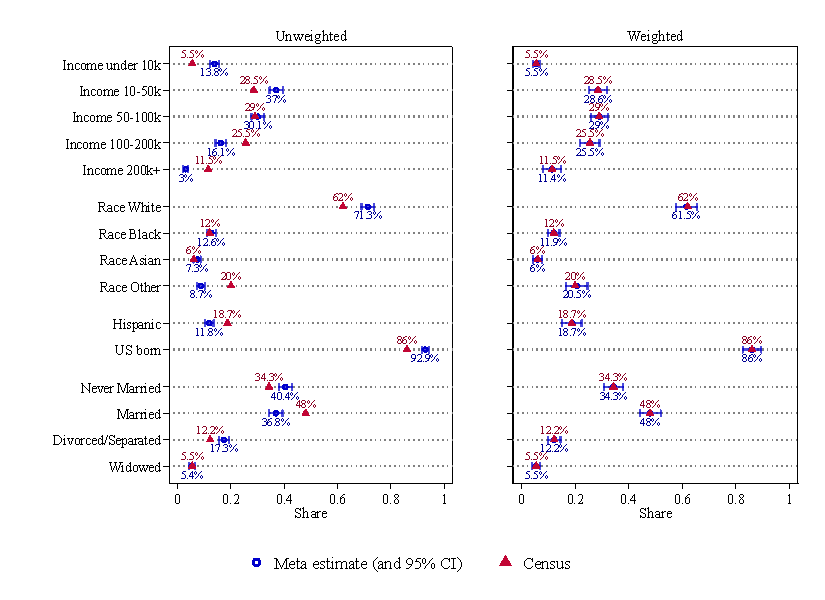
\includegraphics[width=11cm]{Figures/demographics.pdf}
\end{figure}
\end{frame}


\begin{frame}
\frametitle{US Study Results: Political Preferences}
\vspace{-0.2cm}
\begin{figure}[H]
\includegraphics[width=11cm]{Figures/gss_voting.pdf}
\end{figure}
\end{frame}



%\section{Average recruitment costs}
\begin{frame}[label=costs]
\frametitle{Average recruitment costs per country}
\begin{table}[H]
\begin{tabular}{llrlrrl}

\toprule
 & Country & Strata & Max CTR & Reach & Respondents & Average Cost \\
\midrule
0 & India & 24 & 5.09\% & 873653 & 9130 & \$0.24 \\
1 & Libya & 176 & 27.1\% & 1000294 & 8338 & \$0.3 \\
2 & Labanon & 48 & 15.03\% & 1370234 & 17399 & \$0.57 \\
3 & Jordan & 192 & 10.05\% & 2223793 & 17223 & \$0.6 \\
4 & Iraq & 144 & 8.58\% & 4280255 & 16015 & \$0.61 \\
5 & Serbia & 48 & 13.58\% & 985109 & 13995 & \$0.67 \\
6 & Nigeria & 23 & 6.42\% & 145437 & 2393 & \$0.75 \\
7 & US & 10 & 13.61\% & 16849 & 1118 & \$0.85 \\
8 & US & 4 & 6.9\% & 10616 & 316 & \$0.87 \\
9 & Haiti & 16 & 10.0\% & 1218842 & 10491 & \$0.94 \\
10 & Honduras & 144 & 7.4\% & 909597 & 4922 & \$0.95 \\
\bottomrule
\end{tabular}
\end{table}
\end{frame}

\begin{frame}
\frametitle{Average recruitment costs per country}
\begin{table}[H]
\begin{tabular}{llrlrrl}

\toprule
 & Country & Strata & Max CTR & Reach & Respondents & Average Cost \\
\midrule
11 & Lebanon & 48 & 13.82\% & 1650052 & 14354 & \$1.03 \\
12 & Papa NG & 64 & 8.71\% & 118980 & 1825 & \$1.46 \\
13 & Iraq & 80 & 8.27\% & 5616663 & 6520 & \$1.55 \\
14 & US & 14 & 6.14\% & 120647 & 2553 & \$1.66 \\
15 & Ukraine & 64 & 5.17\% & 648512 & 2394 & \$1.69 \\
16 & Kyrgyzstan & 24 & 9.63\% & 489054 & 3004 & \$1.76 \\
17 & Djibouti & 16 & 10.84\% & 313493 & 2252 & \$2.19 \\
18 & Kosovo & 56 & 19.93\% & 663059 & 6084 & \$2.46 \\
19 & Chad & 32 & 7.59\% & 327048 & 2305 & \$2.64 \\
20 & Jamaica & 16 & 15.03\% & 482097 & 4105 & \$2.72 \\
21 & Belize & 24 & 9.1\% & 43684 & 264 & \$2.89 \\
\bottomrule
\end{tabular}
\end{table}
\end{frame}

\begin{frame}
\frametitle{Average recruitment costs per country}
\vspace*{-0.1cm}
\begin{table}[H]
\begin{tabular}{llrlrrl}

\toprule
 & Country & Strata & Max CTR & Reach & Respondents & Average Cost \\
\midrule
22 & Serbia & 1 & 6.75\% & 342403 & 1737 & \$2.99 \\
23 & Macedonia & 32 & 24.58\% & 384956 & 3156 & \$3.19 \\
24 & Romania & 200 & 9.31\% & 785811 & 1863 & \$3.23 \\
25 & Macedonia & 32 & 25.17\% & 538295 & 4565 & \$3.26 \\
26 & Jordan & 96 & 7.14\% & 1304979 & 2146 & \$3.72 \\
27 & US & 16 & 3.93\% & 241134 & 1429 & \$4.55 \\
28 & Nigeria & 120 & 7.75\% & 563939 & 177 & \$5.55 \\
29 & Bulgaria & 8 & 3.91\% & 170205 & 170 & \$6.16 \\
30 & Cameroon & 80 & 11.85\% & 1427793 & 1712 & \$6.72 \\
31 & India & 160 & 5.77\% & 3526970 & 1639 & \$7.85 \\
32 & Gambia & 2 & 5.86\% & 279008 & 697 & \$11.07 \\
\bottomrule
\end{tabular}
\end{table}
\vspace{-0.1cm}
\hyperlink{conclusions}{\beamerskipbutton{Back}}

\end{frame}



\end{document}

%------------------------------------------------
